\chapter{Vývoj zařízení - Konstrukce}
\label{5-vyvoj-zarizeni-konstrukce}
V~této kapitole bude vysvětleno zapojení jednotlivých komponentů, které byly pop\-sány v~předchozí kapitole. Dále bude popsán návrh desky plošných spojů (\zk{DPS}), jenž byl vyhotoven v~softwaru Autodesk EAGLE. Bude vysvětleno, jak byla \zk{DPS} osazena jednotlivými komponenty. Nakonec bude popsáno, jak byl vytvořen prototyp výsledného zařízení.

\section{Schéma zapojení}
Arduino Uno disponuje různými typy pinů, které lze využít k~různým účelům. Při zapojování jednotlivých komponentů je důležité zohlednit specifickou funkcionalitu jednotlivých pinů. Nelze totiž připojit součástky na libovolné piny, ale je nutné je zapojit na piny, které disponují potřebnou funkcionalitou. Jeden pin může mít více funkcí najednou. Piny Arduina mohou sloužit například jako digitální vstupy/výstupy, analogové vstupy, \zk{PWM} (analogové výstupy s~modulací šířky pulzu), RX a TX pro sériovou komunikaci, SDA a SCL pro I\(^2\)C komunikaci nebo jako MISO, MOSI, CLK, a CS pro SPI komunikaci \cite{arduino}.

\begin{figure}[H]
	\centering
	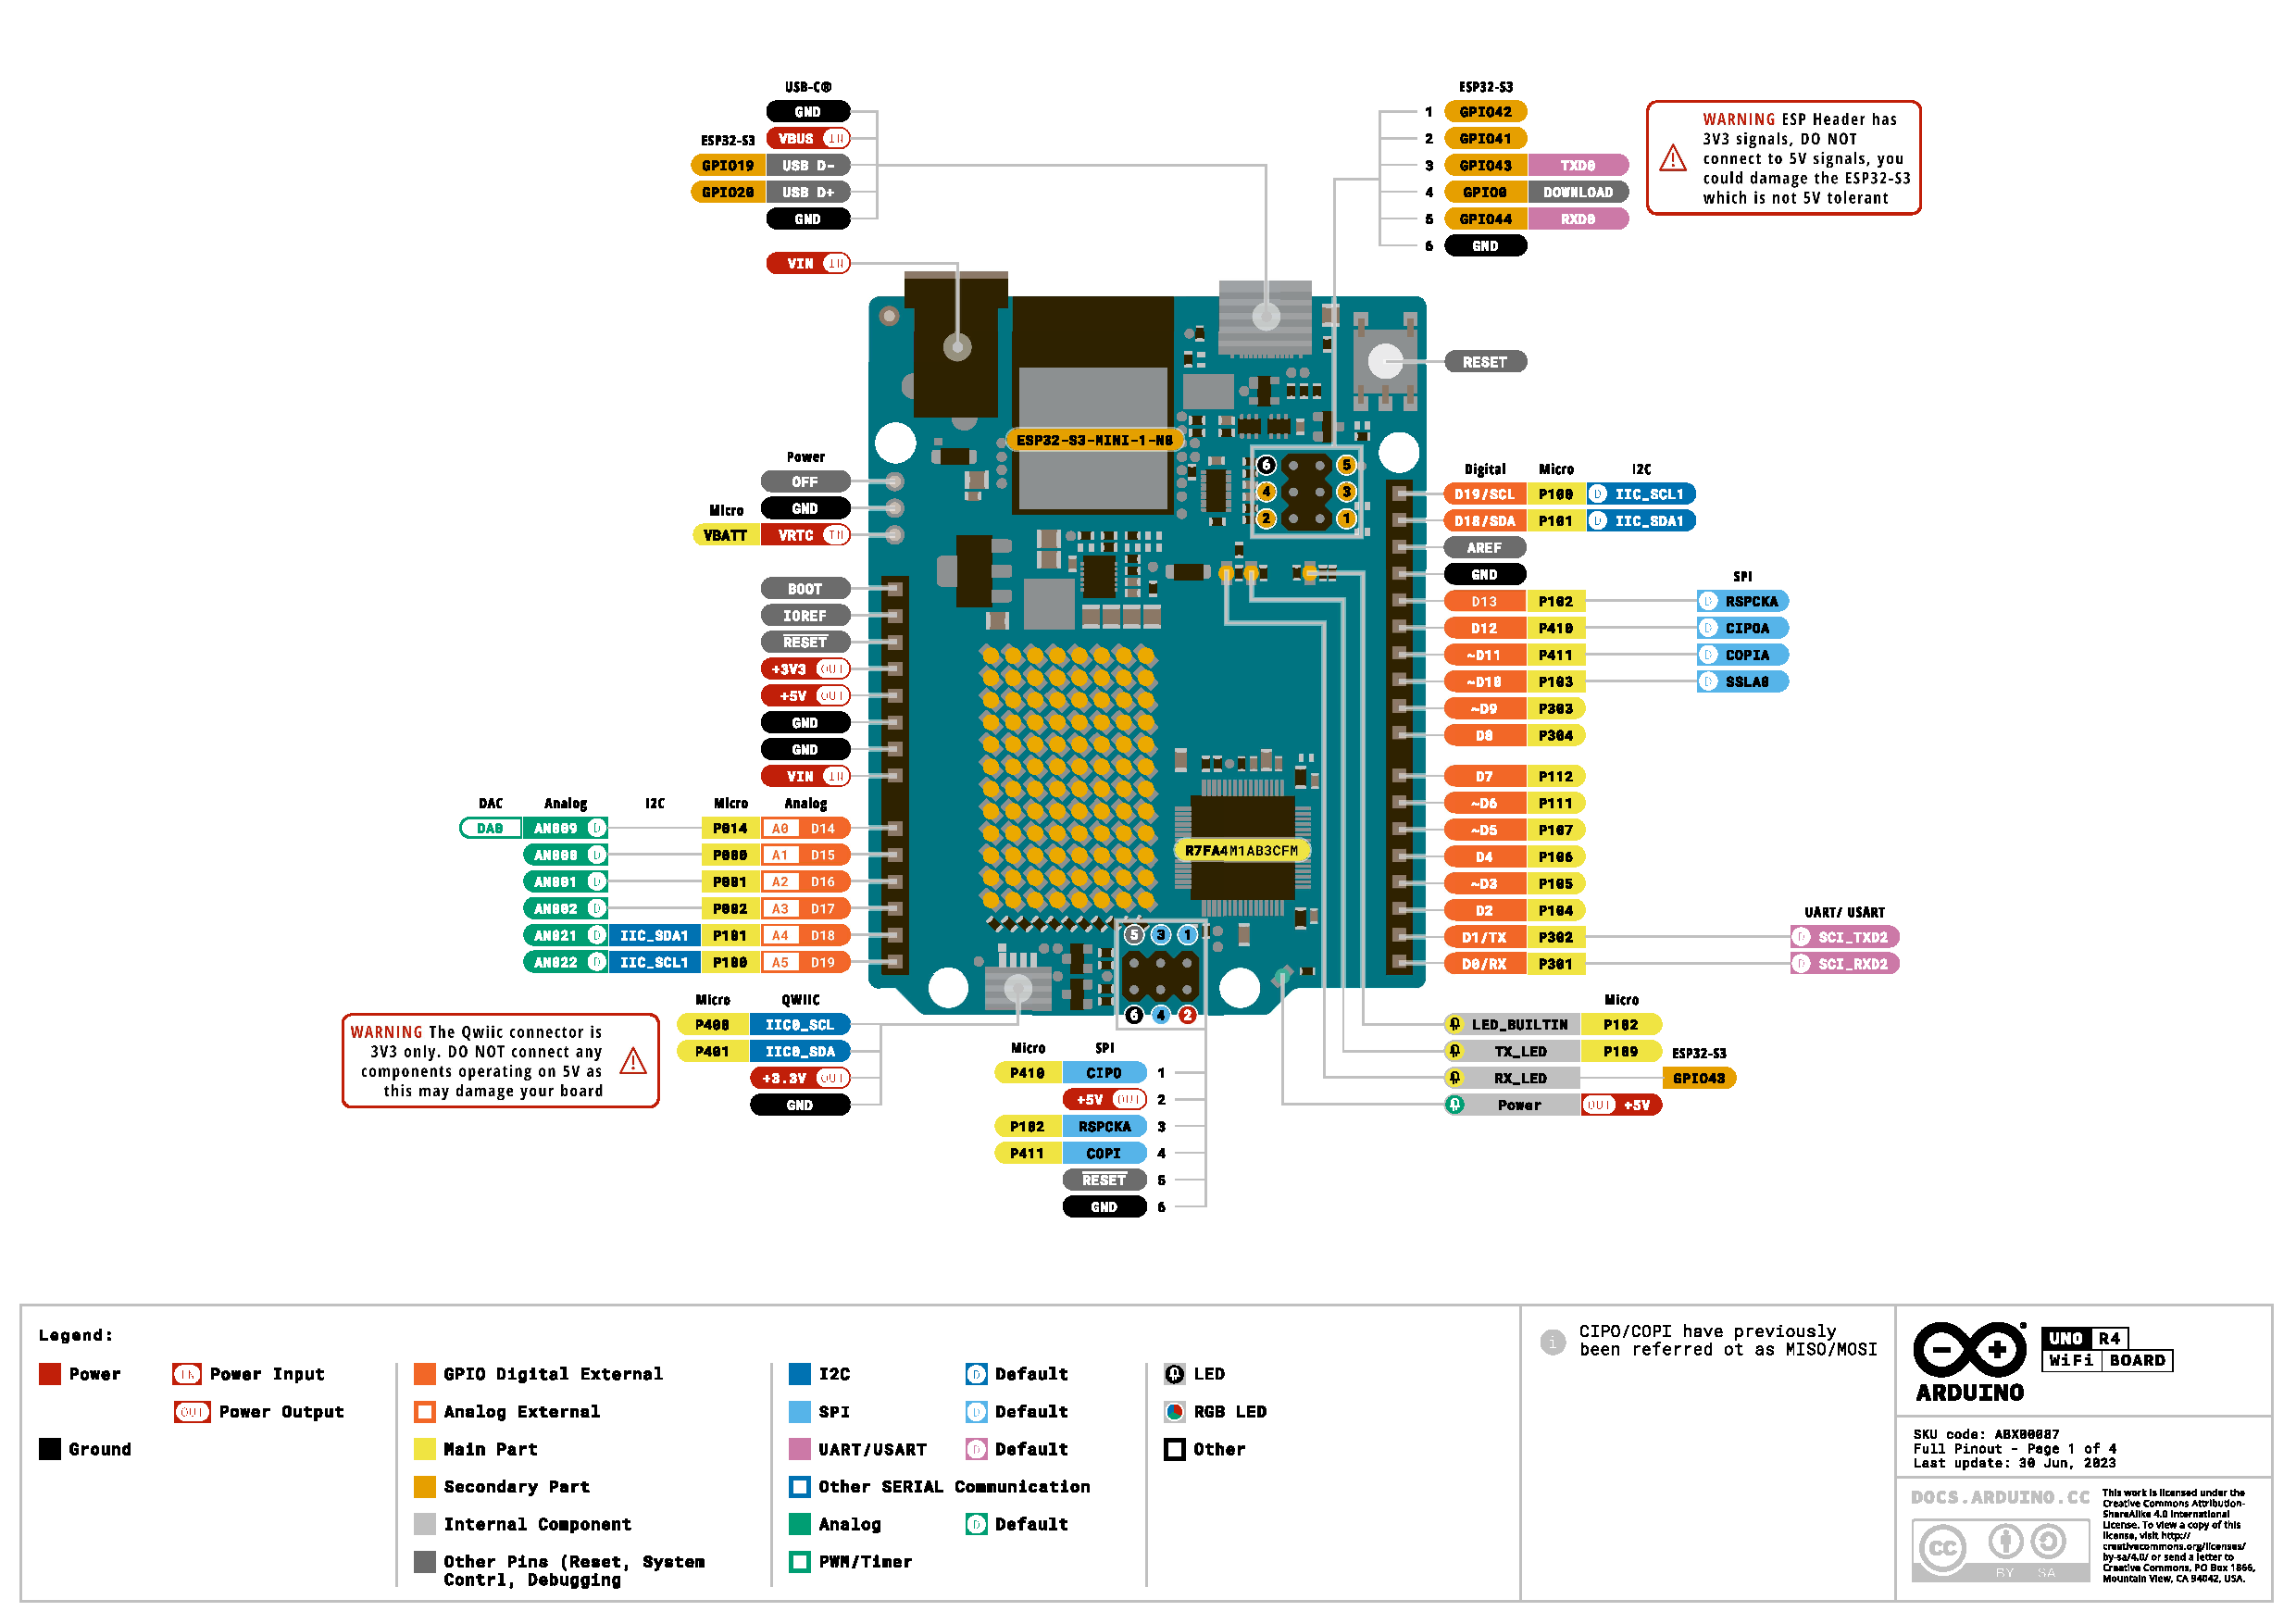
\includegraphics[width=14.9cm]{images/pinout_rotated.pdf}
	\caption{Výstupy pinů pro Arduino UNO R4 \cite{arduino}}
\end{figure}

Schéma zapojení bylo vyhotoveno v~softwaru Autodesk Eagle. nejprve bylo \text{vyhotoveno} schéma zapojení pro Arduino UNO R3 podle toho, jak byly jednotlivé komponenty zapojeny v~rámci testování jejich funkčnosti. Toto schéma zapojení sloužilo jako podklad pro tvorbu desky plošných spojů (\zk{DPS}). Arduino UNO R3 však nedisponuje dostatečnou kapacitou paměti k~tomu, aby mohlo \text{obsluhovat} všechny plánované komponenty. Pro finální zařízení, které bude disponovat plnou funkcionalitou, bylo proto zvoleno Arduino UNO R4. Vzhledem k~tomu, že Arduino UNO R4 má lehce odlišné rozvržení pinů oproti verzi R3, bylo nutné vyhotovit nové schéma zapojení a podle něj i novou \zk{DPS}. Nové schéma zapojení se povedlo navrhnout tak, že nová \zk{DPS} je kompatibilní s~oběma verzemi Arduina UNO (R3 i R4).

\begin{figure}[H]
	\centering
	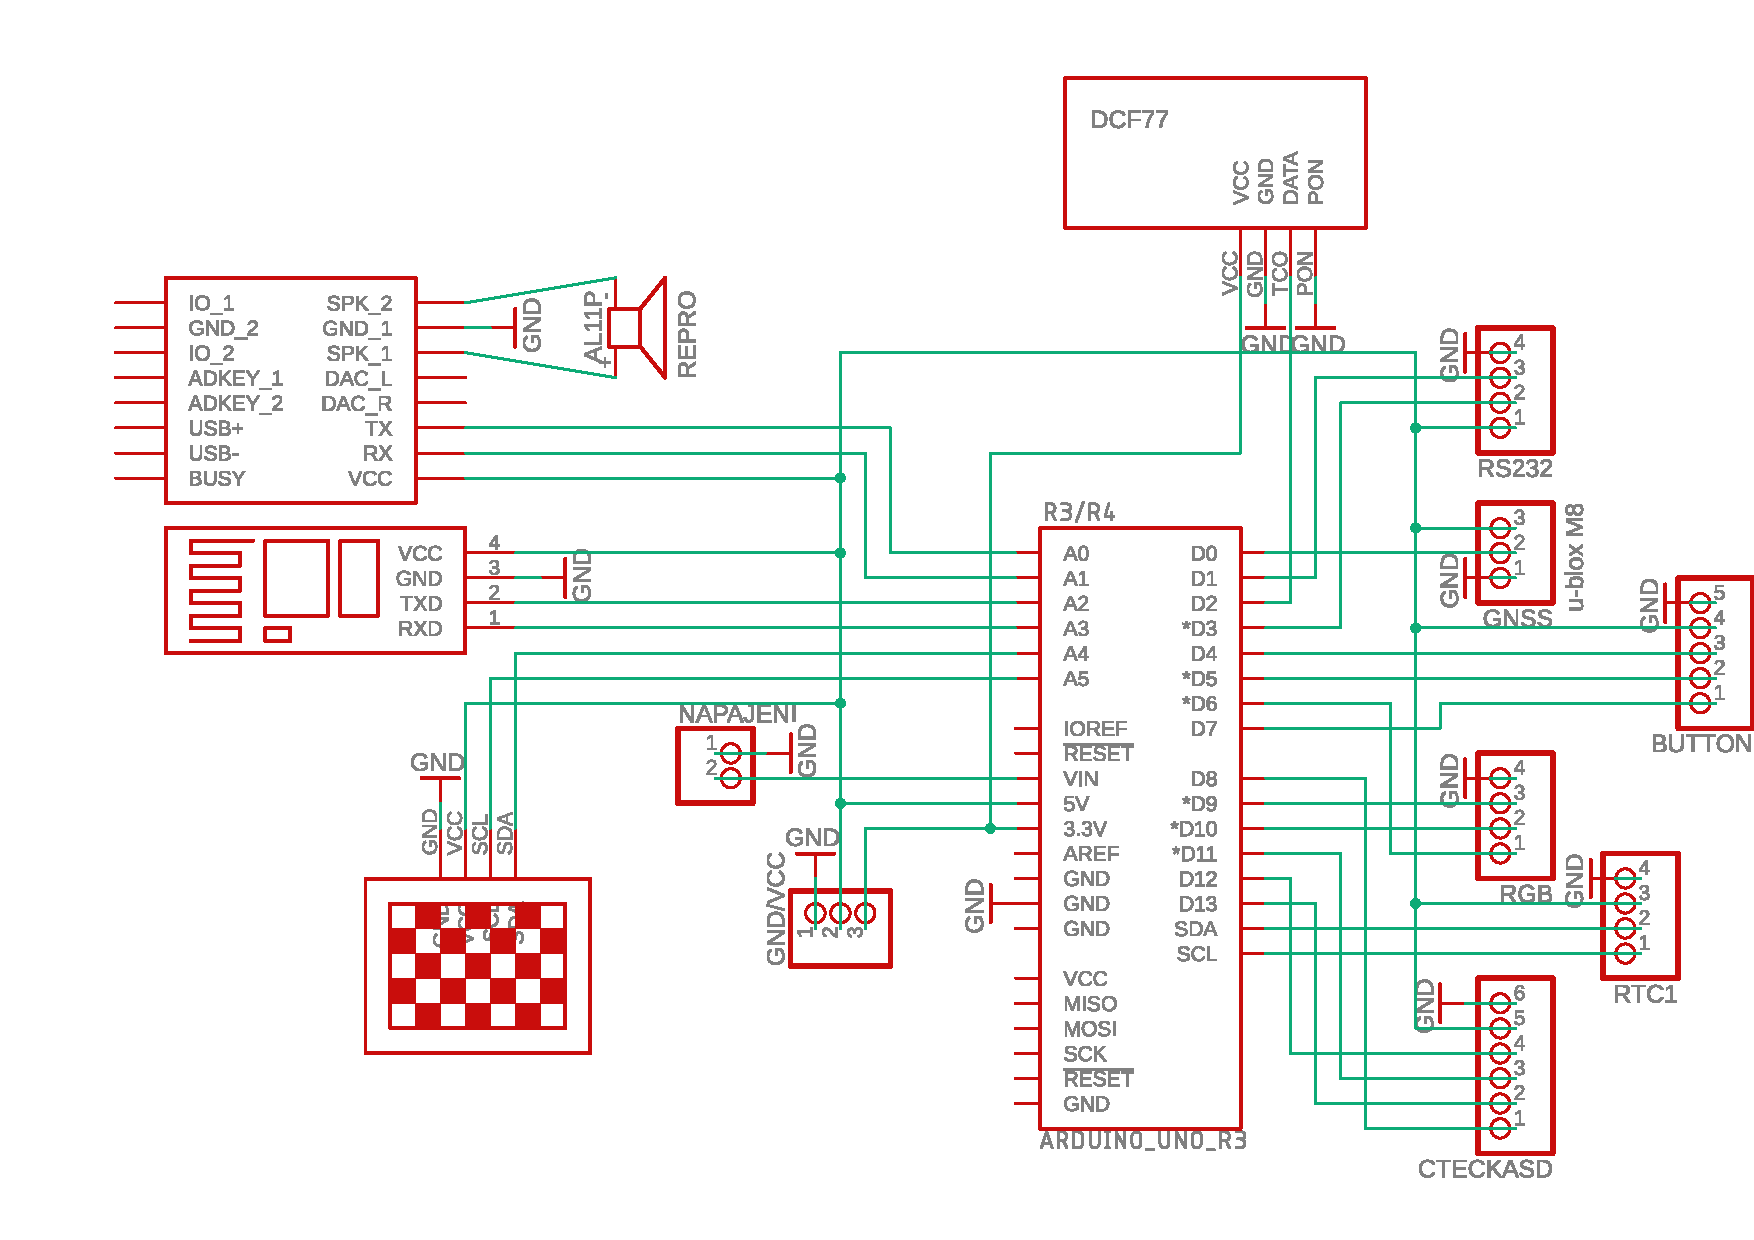
\includegraphics[width=14.1cm]{images/schema_zapojeni.pdf}
	\caption{Schéma zapojení komponentů pro Arduino Uno}
\end{figure}

\subsubsection*{Přijímač časového signálu DCF77}
Přijímač poskytuje digitální signál, který odpovídá dekódovaným bitům časového kódu.
Tento digitální signál je pak k~dispozici na výstupním pinu přijímače (obvykle označeném jako TCO nebo DATA), který je potřeba připojit k~digitálnímu vstupu Arduina.
\begin{itemize}
    \tiny
    \setlength{\itemsep}{0pt} 
    \item VCC $\rightarrow$ 3.3V
    \item GND $\rightarrow$ GND
    \item PON $\rightarrow$ GND
    \item TCO $\rightarrow$ D2
\end{itemize}

\subsubsection*{GNSS přijímač u-blox NEO}
Komunikace s~Arduinem probíhá pomocí sériové komunikace TTL přes rozhraní UART. Je nutné připojit přijímač k~pinům Arduina, které tuto komunikaci umožňují.
 \begin{itemize}
     \tiny
     \setlength{\itemsep}{0pt} 
     \item VCC $\rightarrow$ 5V 
     \item GND $\rightarrow$ GND
     \item TX  $\rightarrow$ D0
 \end{itemize}

    
\subsubsection*{Tlačítko (rotační enkodér)}
Rotační enkodér poskytuje digitální signály, které odpovídají jeho otáčení a stisknutí tlačítka. Tyto signály lze číst pomocí digitálních pinů Arduina, které mohou sloužit jako digitální vstupy.
\begin{itemize}    
    \tiny
    \setlength{\itemsep}{0pt} 
    \item VCC $\rightarrow$ GND
    \item GND $\rightarrow$ 5V
    \item CLK $\rightarrow$ D6
    \item DT  $\rightarrow$ D5
    \item SW  $\rightarrow$ D4
\end{itemize}

\subsubsection*{OLED displej}
OLED displej využívá i\(^2\)C komunikaci a je tedy potřeba jej připojit k~pinům, které ji podporují.
\begin{itemize}
    \tiny
    \setlength{\itemsep}{0pt} 
    \item VCC $\rightarrow$ 5V 
    \item GND $\rightarrow$ GND
    \item SDA $\rightarrow$ A4
    \item SCL $\rightarrow$ A5 
\end{itemize}

\subsubsection*{Hlasový modul}
Hlasový modul využívá sériovou komunikaci. Kvůli nedostatku sériových pinů na Arduinu UNO je použita knihovna SoftwareSerial, která umožňuje emulovat \text{sériovou} komunikaci pomocí některých pinů, které nejsou primárně určeny pro sériovou komu\-nikaci.
\begin{itemize}
    \tiny
    \setlength{\itemsep}{0pt} 
    \item VCC $\rightarrow$ 5V 
    \item GND $\rightarrow$ GND
    \item TX  $\rightarrow$ RX 
    \item RX  $\rightarrow$ TX
    \item SPK1 $\rightarrow$ reproduktor (+)
    \item SPK2 $\rightarrow$ reproduktor (-)
\end{itemize}

\subsubsection*{RGB LED}
Pro ovládání jasu světla jednotlivých barev, lze využít piny s~podporou pulzně šířkové modulace (\zk{PWM}), označené symboly „\(\sim \)“.
\begin{itemize}
    \tiny
    \setlength{\itemsep}{0pt} 
    \item R $\rightarrow$ \(\sim \)D9
    \item G $\rightarrow$ \(\sim \)D10
    \item B $\rightarrow$ \(\sim \)D11
    \item GND $\rightarrow$ GND
\end{itemize}

\subsubsection*{Bluetooth modul HC-05}
Bluetooth modul HC-05 využívá sériovou komunikaci, ale Arduino UNO nemá dosta\-tečný počet sériových pinů. Proto jsou využity piny, které umožňují softwarovou emulaci sériové komunikace obdobně jako u~hlasového modulu.
\begin{itemize}
    \tiny
    \setlength{\itemsep}{0pt} 
    \item VCC $\rightarrow$ 5V 
    \item GND $\rightarrow$ GND
    \item TX  $\rightarrow$ RX 
    \item RX  $\rightarrow$ TX 
\end{itemize}

\section{Návrh DPS}
Návrh \zk{DPS} byl vyhotoven v~softwaru Autodesk Eagle. Propojení mezi komponenty vycházeli z~již vytvořeného schématu zapojení. Bylo navrženo rozmístění komponentů na \zk{DPS}. Pomocí funkce „Autorouter“ byly automaticky vygenerovány optimální trasy spojů. Dále byl vyhotoven „gerberfile“. Ten slouží jako podklad pro výrobu. Výroba \zk{DPS} může být provedena amatérsky. K~tomu je potřeba speciální vybavení a určitá zručnost zhotovitele. Vzhledem k~náročnosti výroby kvalitní \zk{DPS} byla zvolena možnost nechat ji vyrobit profesionální firmou, na základě předloženého „gerberfile“. Tím je zajištěno, že je \zk{DPS} kvalitní a spolehlivá.

\begin{figure}[H]
	\centering
	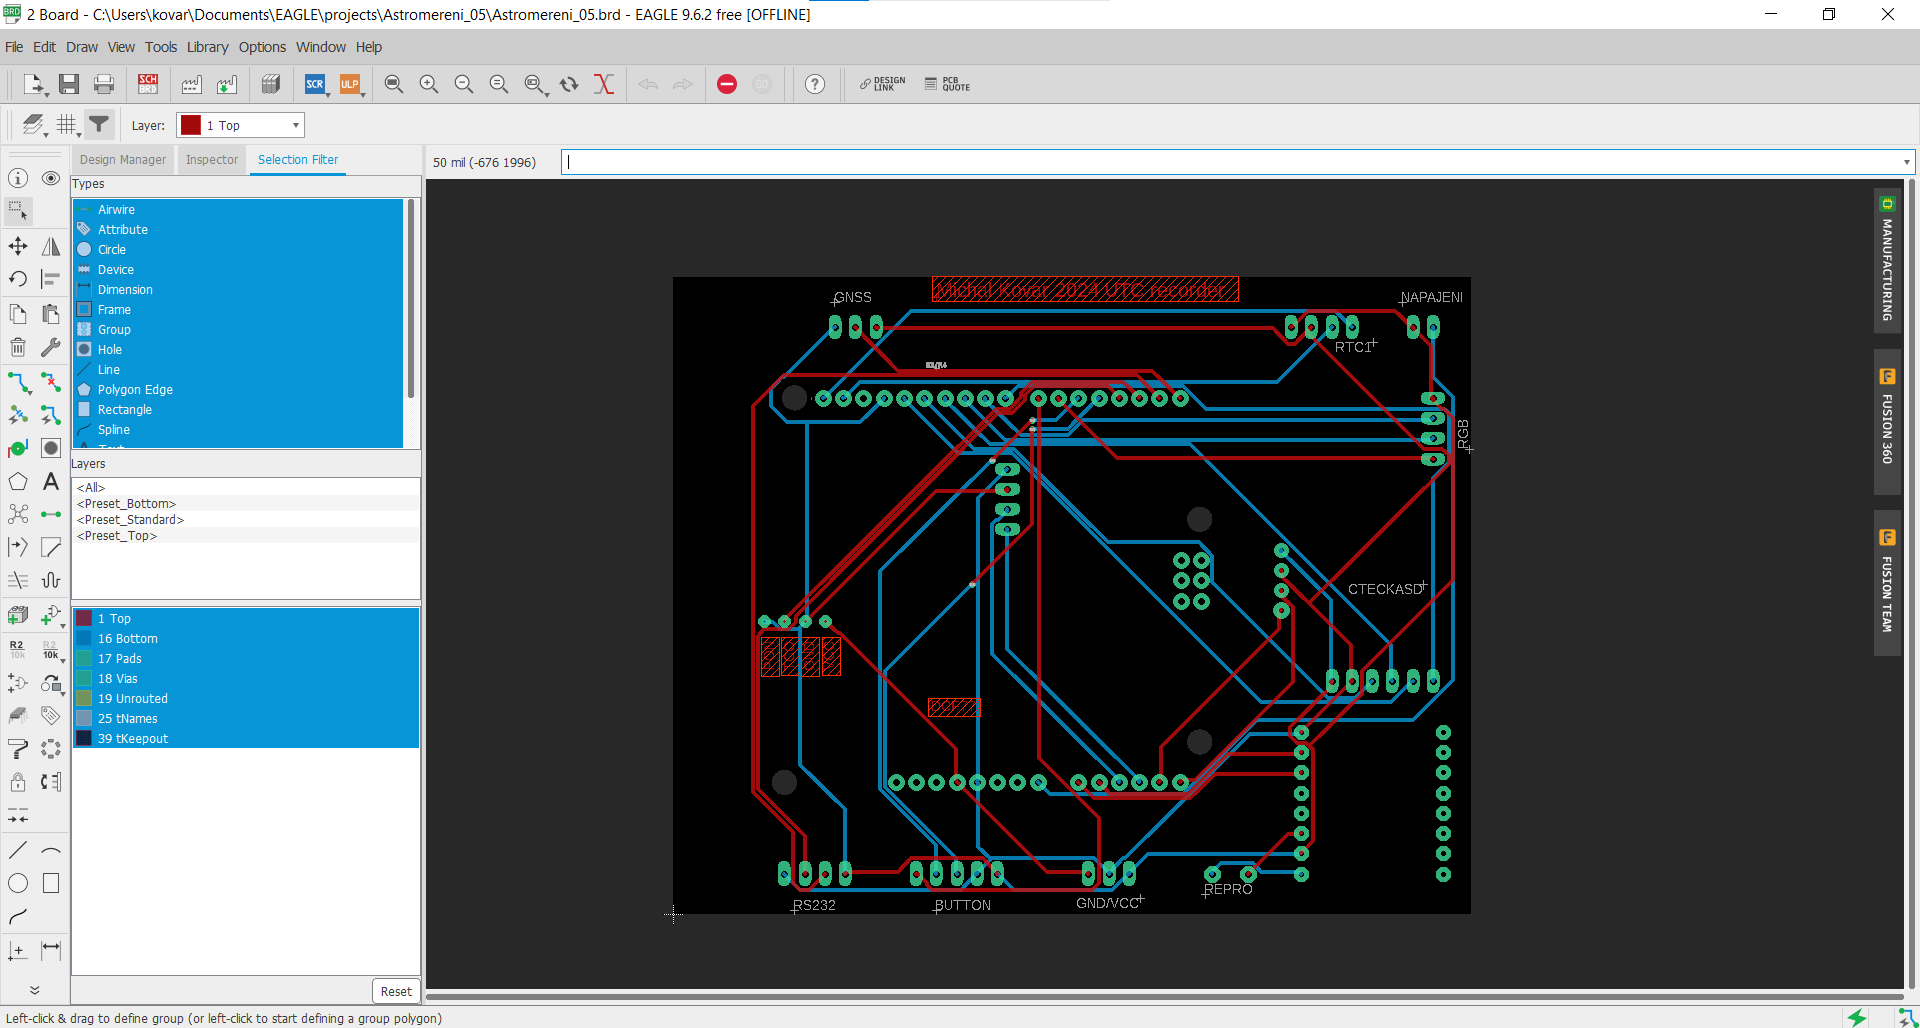
\includegraphics[width=15cm]{images/komponenty/EAGLE_NAVRH_DPS.png}
	\caption{Ukázka návrh DPS v~softwaru Autodesk Eagle}
\end{figure}

\section{Sestavení výsledného zařízení}
Deska plošných spojů byla navržena tak, aby společně s~komponenty k~ní připojenými bylo výsledné zařízení co nejkompaktnější. K~desce byly připájeny další komponenty anebo patice a hřebínky, do kterých budou komponenty zapojeny, aby bylo možné některé komponenty v~případě potřeby odpojit nebo vyměnit. Některé součástky, jako tlačítka a displej byly připojeny k~desce pomocí kabelů. To umožňuje snadné umístění těchto součástek na vnější část krabičky. Kabely lze snadno odpojit pro případ, že by bylo zařízení potřeba rozebrat například z~důvodu výměny nějakého komponentu. Napájení zařízení je řešeno pomocí 9~V~baterie, která je propojená s~piny VIN a GND Arduina.

\begin{figure}[H]
	\centering
	\includegraphics[width=6.8cm]{images/komponenty/Osazená_DPS.jpg}
	\caption{Ukázka osazené DPS pro prototyp zařízení}
\end{figure}

Nakonec byly všechny komponenty integrovány do krabičky, která slouží jako tělo zařízení (astrochronografu). Tělo prototypu zařízení založeného na Arduinu UNO R3 bylo provizorně vytvořeno ze svačinové krabičky, která svými rozměry poměrně dobře vyhovuje potřebám zařízení. Svačinová krabička byla jako tělo zařízení využita z~důvodu toho, že je snadno dostupná a není potřeba ji speciálně vyrábět, zároveň je její výhodou vodotěsnost a průhlednost. V~budoucnu je v~plánu vytvořit vlastní tělo zařízení, které bude kompaktnější a bude přesně vyhovovat účelům zařízení. Do krabičky byly vyvrtány a vyřezány díry pro displej, konektory a tlačítka, které jsou utěsněny silikonem, aby byla zachována vodotěsnost celého zařízení.

\begin{figure}[H]
	\centering
	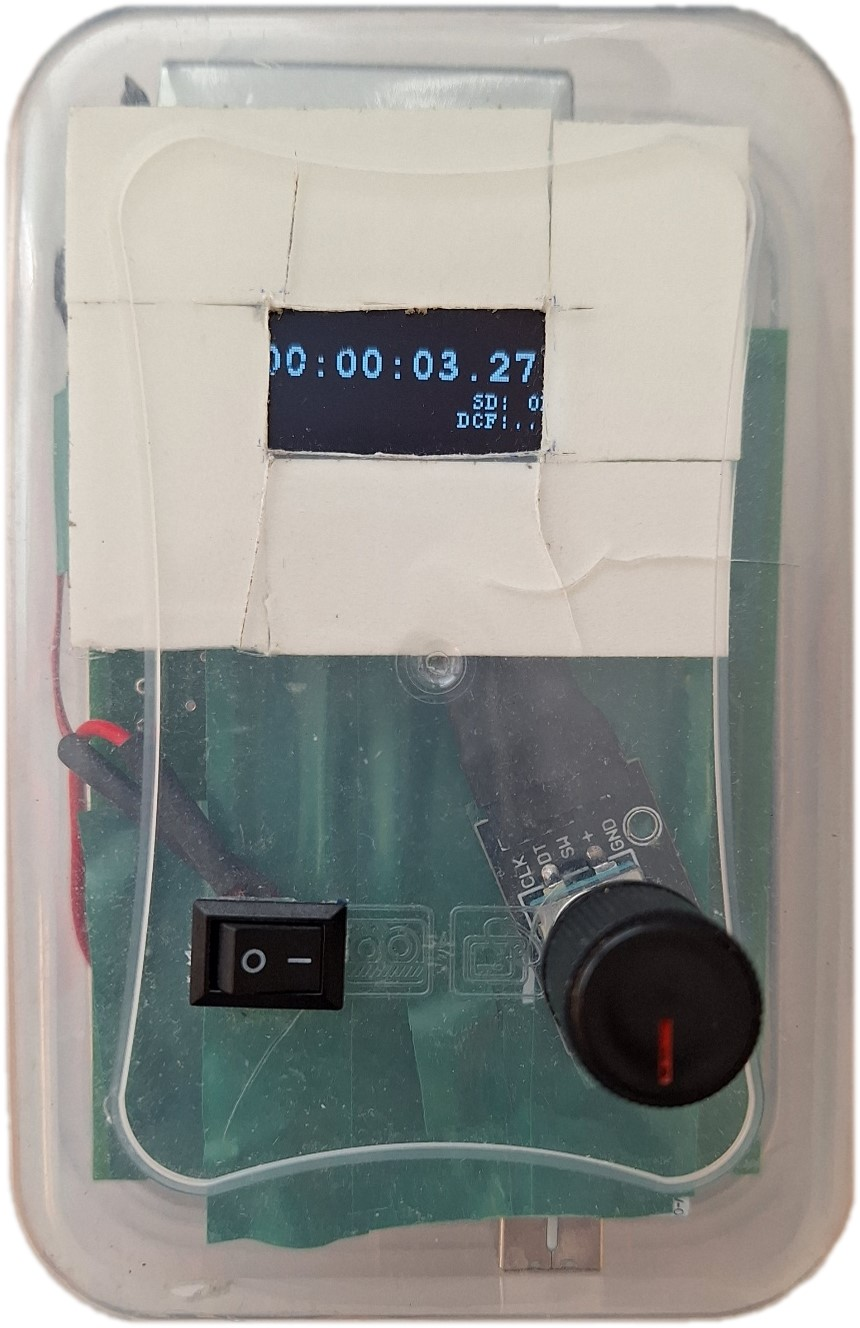
\includegraphics[width=10cm]{images/komponenty/prototyp2.jpg}
	\caption{Prototyp zařízení}
\end{figure}